\documentclass[12pt, a4paper]{article}

%\usepackage[urlcolor=blue]{hyperref}

\usepackage[disable]{todonotes}
\usepackage{todonotes}

\usepackage{booktabs}
\usepackage{pbox}

\usepackage{listings}
\usepackage{amsmath}%
\usepackage{amsfonts}%
\usepackage{amssymb}%
\usepackage{graphicx}
\usepackage[miktex]{gnuplottex}
\ShellEscapetrue
\usepackage{epstopdf}
\usepackage{longtable}
\usepackage{floatrow}
\usepackage{minted}
\usepackage{textcomp}
\usepackage{color,soul}
\usepackage[font={small,it}]{caption}
\floatsetup[listing]{style=Plaintop}
\usepackage[utf8]{inputenc}

% Turn off indentation but allow \indent command to still work.
\newlength\tindent
\setlength{\tindent}{\parindent}
\setlength{\parindent}{0pt}
\renewcommand{\indent}{\hspace*{\tindent}}

\addtolength{\textwidth}{0.8in}
\addtolength{\oddsidemargin}{-.4in}
\addtolength{\evensidemargin}{-.4in}
\addtolength{\textheight}{1.6in}
\addtolength{\topmargin}{-.8in}

\usepackage{longtable,supertabular}
\usepackage{footnote}
\usepackage{listings}
\lstset{
  frame=top,frame=bottom,
  basicstyle=\ttfamily,
  language=XML,
  tabsize=2,
  belowskip=2\medskipamount
}

%\usepackage{float}
\usepackage{tabu}
\tabulinesep=1.0mm
\restylefloat{table}

\usepackage{siunitx}
\usepackage{hyperref}
\hypersetup{
	colorlinks=true, %set true if you want colored links
	linktoc=all,     %set to all if you want both sections and subsections linked
	linkcolor=blue,  %choose some color if you want links to stand out
}

%\usepackage[colorlinks=true]{hyperref}

\renewcommand\P{\ensuremath{\mathbb{P}}}
\newcommand\E{\ensuremath{\mathbb{E}}}
\newcommand\Q{\ensuremath{\mathbb{Q}}}
\newcommand\I{\mathds{1}}
\newcommand\F{\ensuremath{\mathcal F}}
\newcommand\V{\ensuremath{\mathbb{V}}}
\newcommand\YOY{{\rm YOY}}
\newcommand\Prob{\ensuremath{\mathbb{P}}}
\newcommand{\D}[1]{\mbox{d}#1}
\newcommand{\NPV}{\mathit{NPV}}
\newcommand{\CVA}{\mathit{CVA}}
\newcommand{\DVA}{\mathit{DVA}}
\newcommand{\FVA}{\mathit{FVA}}
\newcommand{\COLVA}{\mathit{COLVA}}
\newcommand{\FCA}{\mathit{FCA}}
\newcommand{\FBA}{\mathit{FBA}}
\newcommand{\KVA}{\mathit{KVA}}
\newcommand{\MVA}{\mathit{MVA}}
\newcommand{\PFE}{\mathit{PFE}}
\newcommand{\EE}{\mathit{EE}}
\newcommand{\EPE}{\mathit{EPE}}
\newcommand{\ENE}{\mathit{ENE}}
\newcommand{\PD}{\mathit{PD}}
\newcommand{\LGD}{\mathit{LGD}}
\newcommand{\DIM}{\mathit{DIM}}
\newcommand{\bs}{\textbackslash}
\newcommand{\REDY}{\color{red}Y}
\newcommand\enforce{\,\raisebox{0.8 ex}{$\substack{!\\\displaystyle=}$} \,}


\begin{document}

\title{ORE Formula Based Coupon Module}
\author{Quaternion Risk Management}
\date{20 Feburary 2019}
\maketitle

\newpage

%-------------------------------------------------------------------------------
\section*{Document History}

\begin{center}
\begin{supertabular}{|l|l|l|p{7cm}|}
\hline
ORE+ Release & Date & Author & Comment \\
\hline
na & 29 August 2018  & Peter Caspers& initial version\\
1.8.4.0 & 20 February 2019 & Sarp Kaya Acar & add examples \\
\hline
\end{supertabular}
\end{center}

\vspace{3cm}

\newpage

\tableofcontents
\vfill

\textcircled{c} 2019 Quaternion Risk Management Limited.  All rights reserved.
Quaternion\textsuperscript{\textregistered} is a trademark of Quaternion Risk Management Limited and is also registered
at the UK Intellectual Property Office and the U.S. Patent and Trademark Office.  All other trademarks are the property
of their respective owners. Open Source Risk Engine\textsuperscript{\textcircled{c}} (ORE) is sponsored by Quaternion
Risk Management Limited.

\newpage



%-------------------------------------------------------------------------------
\section{Summary}

This document describes the formula based coupon implemented in ORE+.



\section{Methodology}
\label{ssection_FormulaBasedLeg}
\subsection{Introduction}

We consider a generalised structured coupon which at time $T$ pays

\begin{equation} \tau f(R_1(t), \ldots, R_n(t))
\end{equation}

where $\tau$ is the year fraction of the coupon, $R_i$'s are IBOR and/or CMS rates fixed at time $t<T$ and $f$ is a
payoff function. Moreover we assume that the currency of the coupon can be different than the currency of the rates,
i.e. the quanto-payoffs are allowed. For instance, let us consider the below example
%
\begin{equation}
f(R_1, R_2) = 1_{\{R_3>0.03\}}\max\{\min\{9\cdot (R_2-R_1)+0.02,0.08\},0.0\},
\label{eq:FBCpayoff}
\end{equation}
%
with $R_1=$GBP-CMS-2Y, $R_2=$EUR-CMS-10Y, $R_3=$USD-CMS-5Y. With the Formula-Based-Coupon module it is possible to price
such kind of coupons by using the Monte-Carlo simulation technique. In the next section, we will present the underlying
pricing model.

\subsection{Pricing Model}
\label{ssection_FormulaBasedLegPricingModel}
For non-callable structured coupons, we generalise the model in
\cite{brigo}, 13.16.2. We assume the rates
to evolve with a shifted lognormal dynamics under the $T$-forward
measure in the respective currency of $R_i$ as

\begin{equation}\label{lndyn} dR_i = \mu_i (R_i + d_i) dt + \sigma_i
(R_i + d_i) dZ_i
\end{equation}

with displacements $d_i>0$, drifts $\mu_i$ and volatilities $\sigma_i$
or alternatively with normal dynamics

\begin{equation}\label{ndyn} dR_i = \mu_i dt + \sigma_i dZ_i
\end{equation}

for $i=1,\ldots,n$ where in both cases $Z_i$ are correlated Brownian
motions

\begin{equation} dZ_i dZ_j = \rho_{i,j} dt
\end{equation}

with a positive semi-definite correlation matrix $( \rho_{i,j})$. The
drifts $\mu_i$ are determined using given convexity adjustments

\begin{equation} c_i = E^T(R_i(t)) - R_i(0)
\end{equation}

where the expectation is taken in the $T$-forward measure in the
currency of the respective rate $R_i$. Slightly abusing notation $c_i$
can be computed both using a model consistent with \ref{lndyn}
resp. \ref{ndyn} (i.e. a Black76 style model) or also a different
model like e.g. a full smile TSR model to compute CMS
adjustments. While the latter choice formally introduces a model
inconsistency it might still produce more market consistent prices at
the end of the day, since it centers the distributions of the $R_i$
around a mean that better captures the market implied convexity
adjustments of the rates $R_i$ entering the structured coupon payoff.

Under shifted lognormal dynamics the average drift is then given by

\begin{equation} \mu_i = \frac{\log( (R_i(0)+d_i+c_i) / (R_i(0)+d_i)
)}{t}
\end{equation}

and under normal dynamics

\begin{equation} \mu_i = c_i / t
\end{equation}

The NPV $\nu$ of the coupon is now given by

\begin{equation}\label{struccpnnpv} \nu = P(0,T) \tau E^T ( f(R_1(t),
\ldots, R_n(t)) )
\end{equation}

where $P(0,T)$ is the applicable discount factor for the payment time
in the domestic currency and the expectation is taken in the
$T$-forward measure in the domestic currency. To adjust \ref{lndyn}
resp. \ref{ndyn} for the measure change between the currency of $R_i$
and the domestic currency (if applicable), we apply the usual Black
quanto adjustment

\begin{equation}
  \mu_i \rightarrow \mu_i + \sigma_i \sigma_{i,X} \rho_{i,X}
\end{equation}

where $\sigma_{i,X}$ is the volatility of the applicable FX rate and
$\rho_{i,X}$ is the correlation between the Brownian motion driving
the FX process and $Z_i$.

To evaluate the expectation in \ref{struccpnnpv} a Monte Carlo
simulation can be used to generate samples of the distribution of
$(R_1, \ldots, R_n)$, evaluate $f$ on these samples and average the
results.

\section{Parametrisation}

%\subsection{Trade Components}

\subsection{Formula Based Leg Data}

The formula based leg data allows to use complex formulas to describe coupon payoffs. Its {\tt LegType} is {\tt
  FormulaBased}, and it has the data section {\tt FormulaBasedLegData}. It supports IBOR and CMS based payoffs with
quanto and digital features. The following examples shows the definition of a coupon paying a capped / floored cross
currency EUR-GBP CMS Spread contingent on a USD CMS barrier.



The {\tt Index} field supports operations of the following kind:
\begin{itemize}
\item indices like IBOR and CMS indices, and constants as factors,
  spreads and/or cap/floor values;
\item basic operations: $+$, $-$, $\cdot$, $/$;
\item operators gtZero() (greater than zero) and geqZero() (greater than or equal zero) yielding $1$ if the argument is
  $>0$ (resp. $\geq 0$) and zero otherwise
\item functions: abs(), exp(), log(), min(), max(), pow()
\end{itemize}
%
In listing \ref{lst:FBLegdata}, we present the {\tt FormulaBasedLegData} of the payoff in equation \ref{eq:FBCpayoff}.
%
\begin{listing}
\begin{minted}[fontsize=\footnotesize]{xml}
<LegData>
  <LegType>FormulaBased</LegType>
  <Payer>true</Payer>
  <Currency>EUR</Currency>
   ...
  <FormulaBasedLegData>
    <Index>gtZero({USD-CMS-5Y}-0.03)*
              max(min(9.0*({EUR-CMS-10Y}-{GBP-CMS-2Y})+0.02,0.08),0.0)</Index>
    <IsInArrears>false</IsInArrears>
    <FixingDays>2</FixingDays>
  </FormulaBasedLegData>
   ...
</LegData>
\end{minted}
\caption{FormulaBasedLegData configuration.}
\label{lst:FBLegdata}
\end{listing}
%
\section{Pricing Engine settings}

The configuration of the pricing engine for the model introduced in section \ref{ssection_FormulaBasedLegPricingModel}
is given in listing \ref{lst:FBCpricer}.

\begin{itemize}
\item The formula based coupon pricer uses the pricing engine configuration for { \tt CapFlooredIborLeg} and {\tt CMS}.
  For the configuration of these coupon pricers we refer to sections 7.3, 7.7.3 and 7.74 in \cite{oreug}.
\item The parameter \verb+FXSource+ specifies the FX index tag to be used to look up FX-Ibor or FX-CMS correlations, see
  also 7.10.2 in \cite{oreug}.
\end{itemize}
%
\begin{listing}
\begin{minted}[fontsize=\footnotesize]{xml}
  <!-- Formula Based Coupons -->
  <Product type="FormulaBasedCoupon">
    <Model>BrigoMercurio</Model>
    <ModelParameters>
      <Parameter name="FXSource">ECB</Parameter>
    </ModelParameters>
    <Engine>MC</Engine>
    <EngineParameters>
      <Parameter name="Samples">1000</Parameter>
      <Parameter name="Seed">42</Parameter>
      <Parameter name="Sobol">Y</Parameter>
      <Parameter name="SalvageCorrelationMatrix">Y</Parameter>
    </EngineParameters>
  </Product>
\end{minted}
\caption{Pricing engine configuration for formula based coupon pricer.}
\label{lst:FBCpricer}
\end{listing}
%
\section{Market Data}

The relevant market data for the formula based coupon pricer encompasses

\begin{enumerate}
\item rate curves (for index projection and cashflow discounting)
\item cap / floor volatilities (for Ibor coupon pricers in the relevant currencies)
\item swaption volatilities (for CMS coupon pricers in the relevant currencies)
\item correlation curves for the relevant Ibor-Ibor, Ibor-CMS, CMS-CMS, Ibor-FX, CMS-FX pairs
\end{enumerate}

See \cite{oreug} for details on the setup and configuration of this market data.

\section{Examples}

\subsection{CMS Spread}
We demonstrate a single currency Swap (currency EUR, maturity 20y, notional 10m, receive fixed $0.011244\%$ annual, pay
$\max \left\{ \text{CMS-EUR-10Y}- \text{CMS-EUR-1Y}, 0.0 \right \}$ semi-annual).
%
We simulate the exposure with 1000 Monte-Carlo paths by using the formula based coupon pricer and the analytical
CMS-Spread pricer [section 7.10.8, \cite{oreug}]. The number of Monte-Carlo paths in formula based coupon pricer is
1000. EPE profiles with both runs are given in figure \ref{fig:MC1K}. We observed that the run with the formula based
coupon pricer is approximately $2.5$ times slower than the analytical one.
%
\begin{figure}
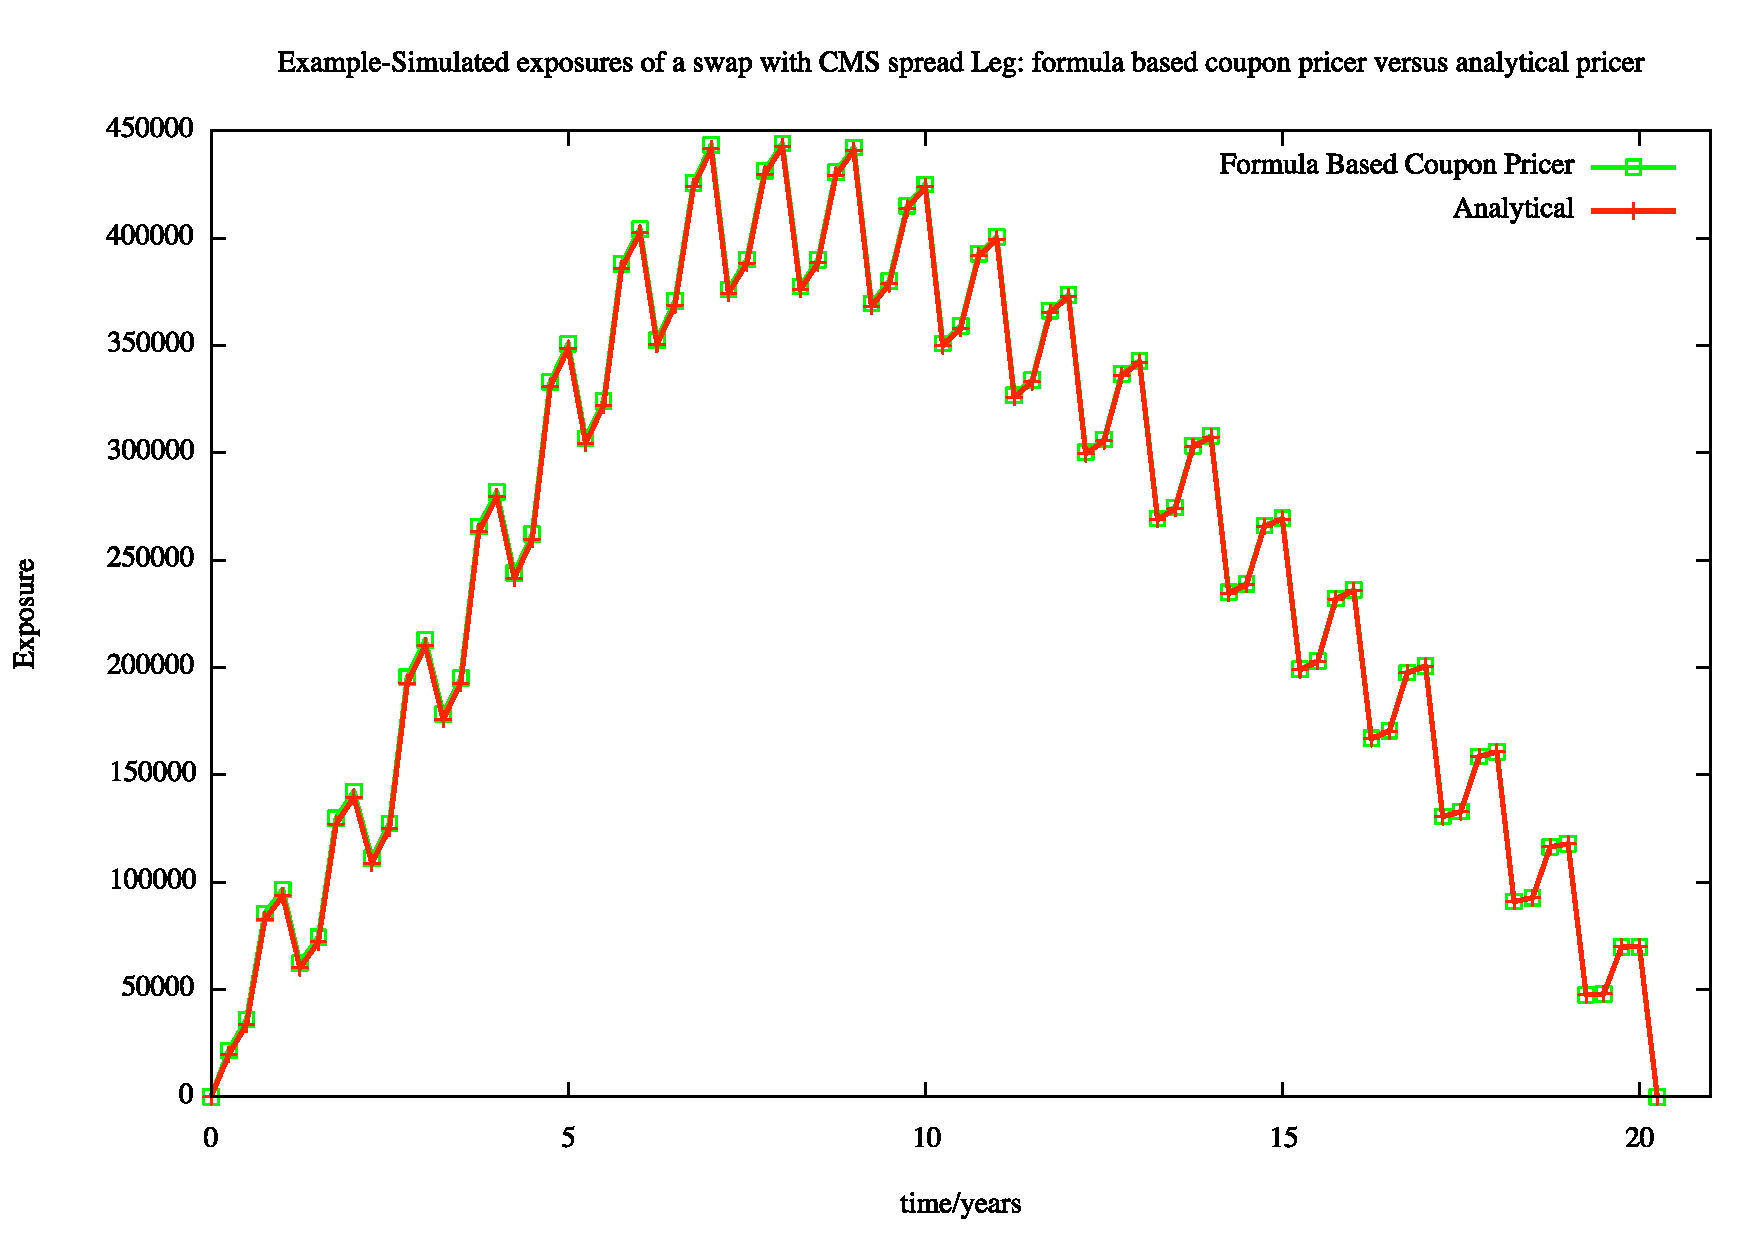
\includegraphics[scale=0.55]{MC1K.pdf}
\caption{20Y EUR interest rate swap with floored CMS spread leg, i.e.
  $\max(\text{EUR-CMS-10Y} - \text{EUR-CMS-1Y},\, $0.5\%$) $ }
\label{fig:MC1K}
\end{figure}

\subsection{Digital CMS Spread}
As a second example, we demonstrate a single currency Swap (currency EUR, maturity 20y, notional 10m, receive fixed
$0.011244\%$ annual, pay
$\left(\text{CMS-EUR-10Y}- \text{CMS-EUR-1Y} \right)+ 0.01 * 1_{\left\{\text{CMS-EUR-10Y}-
    \text{CMS-EUR-1Y}>0.0\right\}} $ semi-annual).

\begin{figure}
  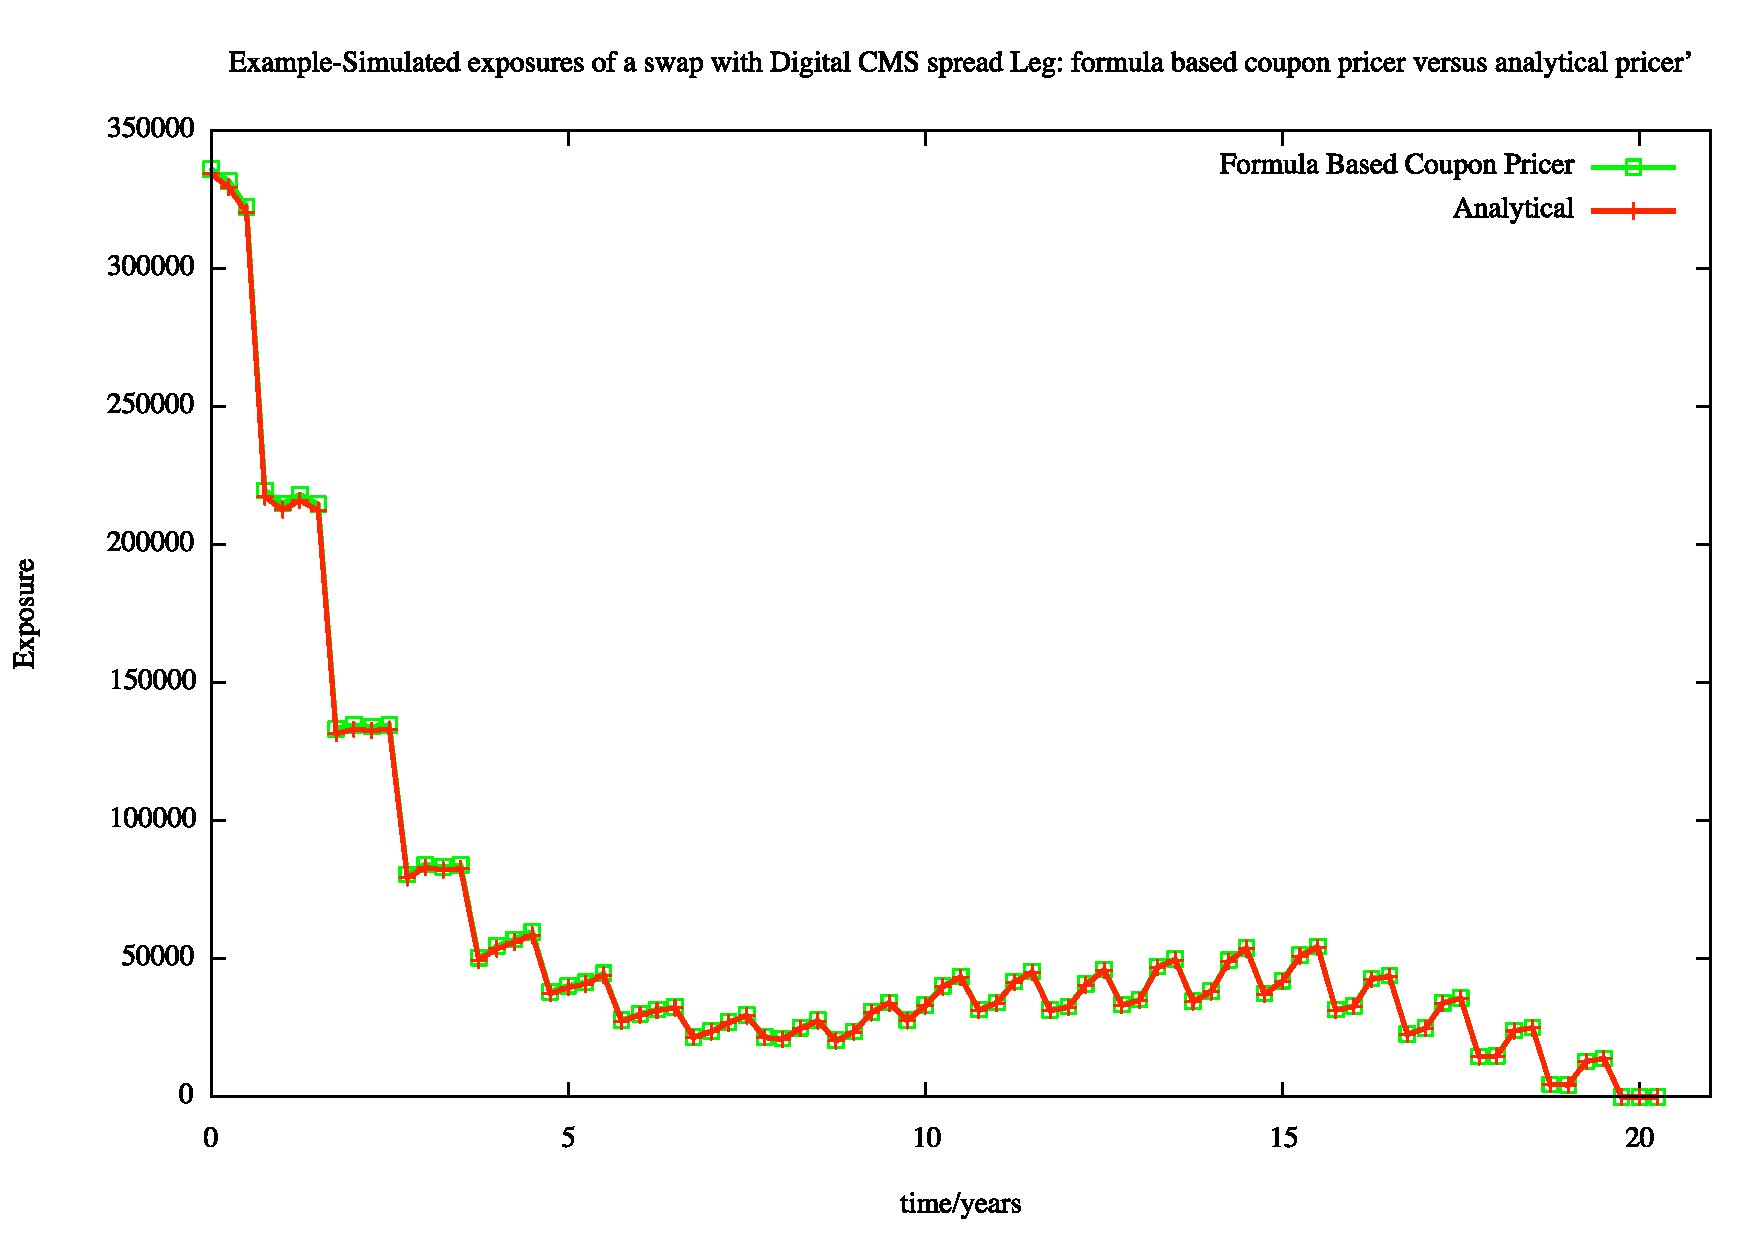
\includegraphics[scale=0.55]{Digital_MC1K_2.pdf}
  \caption{20Y EUR interest rate swap with digital CMS spread leg, i.e.
    $\left(\text{CMS-EUR-10Y}- \text{CMS-EUR-1Y} \right)+ 0.01 * 1_{\left\{\text{CMS-EUR-10Y}-
        \text{CMS-EUR-1Y}>0.0\right\}} $ }
\label{fig:Digital:MC1K}
\end{figure}



\pagebreak
%\appendix
%\section*{Appendices}
%\addcontentsline{toc}{section}{Appendices}
\renewcommand{\thesubsection}{\Alph{subsection}}
%\section{Appendix}

%\subsection{Test}\label{ss_LGM}



\begin{thebibliography}{1}

\bibitem{oreug} ORE User Guide,
  \url{http://www.opensourcerisk.org/documentation/}
% \bibitem{AP}Andersen, Leif B. G., Piterbarg, Vladimir V.: Interest
%   Rate Modeling -- Vol. 3: Products and Risk Management, Atlantic
%   Financial Press, 2010
\bibitem{brigo}Brigo, Damiano; Mercurio, Fabio: Interest Rate Models - Theory and
  Practice, 2nd Edition, Springer, 2006
% \bibitem{Hagan}Hagan, Patrick: Convexity Conundrums, Wilmott, 2003
% \bibitem {Hfb}Heidorn, Schmidt, \textit{LIBOR in Arrears}, 1998, Frankfurt School of Finance
% \bibitem{LSG}Lichters, Roland; Stamm, Roland; Gallgher, Donal: Modern
%   Derivatives Pricing, Palgrave Macmillan, 2015
% \bibitem {Papa}Papaioannou Denis, \textit{Applied Multidimensional
%     Girsanov Theorem}, Electronic copy available at:
%   http://ssrn.com/abstract=1805984 



\end{thebibliography}

\end{document}
